\documentclass[informe.tex]{subfiles}
\begin{document}

La característica principal es la de tener una buena aproximación uniforme en toda la banda de paso. Los parámetros característicos son la constante de riple y el orden, que dependen de los requerimientos de atenuación. Otra característica importante es que la frecuencia de corte es mayor a uno (cuando se tiene la frecuencia normalizada). \newline

%%
\textbf{Función de aproximación:}\newline

Queda definida por
		\[	
		C(\omega ) 	=
		    \begin{cases}
		    		cos(n \cdot cos^{-1}( \omega) )  &
		                          \mbox{, si  } \left| \omega \right| <=1   \\
		    		cosh(n \cdot cosh^{-1}( \omega) )  &
		                          \mbox{, si } \left| \omega \right| >1   
		    \end{cases}
		\]
y para el caso de que la expresión dada se defina en forma recursiva sería:	
		$$
		C(\omega)=
		    \begin{cases}
			    1                                & \mbox{, si } n=0\\
 	      		\omega                           & \mbox{, si } n=1\\
    				2\omega C_{n-1}- C_{n-2}(\omega) & \mbox{, para otro valor de } n
		    \end{cases}
		$$\newline
		   	    		
 \begin{tabular}{p{0.45\textwidth} p{0.5\textwidth}}		
			
			\begin{wrapfigure}{l}{0.9\linewidth}
			\centering
			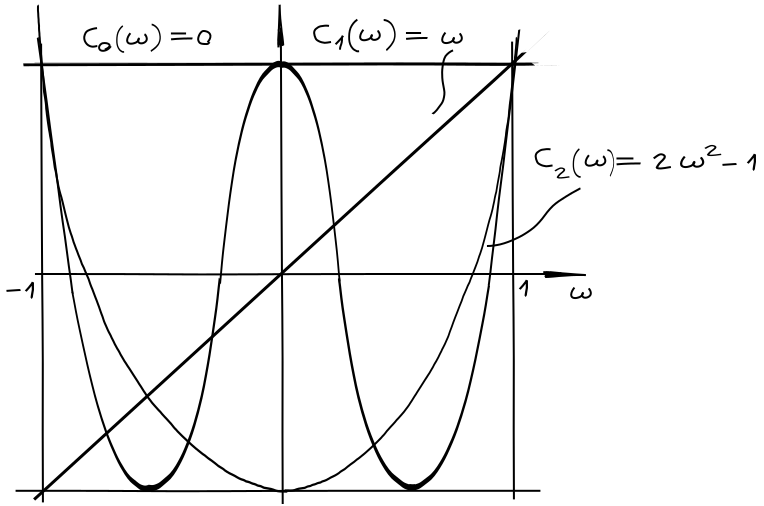
\includegraphics[width=\linewidth]{chebyshev_polinomio.png}
			\caption{Polinomos de Chebyshev}
			\end{wrapfigure}				
			&
			Resumen de propiedades:\newline
			1- Los valores característicos son:
				\[  
					C_n(0)= \begin{cases}
							    0  & \mbox{, si n es impar} \\
 	      						1  & \mbox{, si n es par} 
						    \end{cases}
				 \]
			2- Los ceros están en el intervalo $ \left| \omega \right|<1$.\newline
			3- Dentro del intervalo, $ \left| \omega \right|<=1$, no excede la unidad. \newline
			4- El valor absoluto de la función se incrementa rápidamente para $|\omega|>1$.
		\end{tabular} 
\\\\\\\\\\\\\\\\\\

%%
\textbf{Función de respuesta en frecuencia}\newline	
		\[ \left| H(j\omega) \right|^2 = \frac{1}{ 1 +  \epsilon^2 C_n^2(\omega)  } \]
		
donde $\epsilon$ es la constante de riple, y $C_n(\omega)$ es la función de Chebyshev de orden $n$. En el intervalo  $ \left| \omega \right| \le 1 $ oscilará desde un máximo, en $1$, a un mínimo, en $ \frac{1}{1+\epsilon^2} $, y fuera de este intervalo se aproxima a cero rápidamente.\\

	\begin{tabular}{p{0.45\textwidth} p{0.5\textwidth}}		
			
		\begin{wrapfigure}{l}{0.9\linewidth}
		\centering
		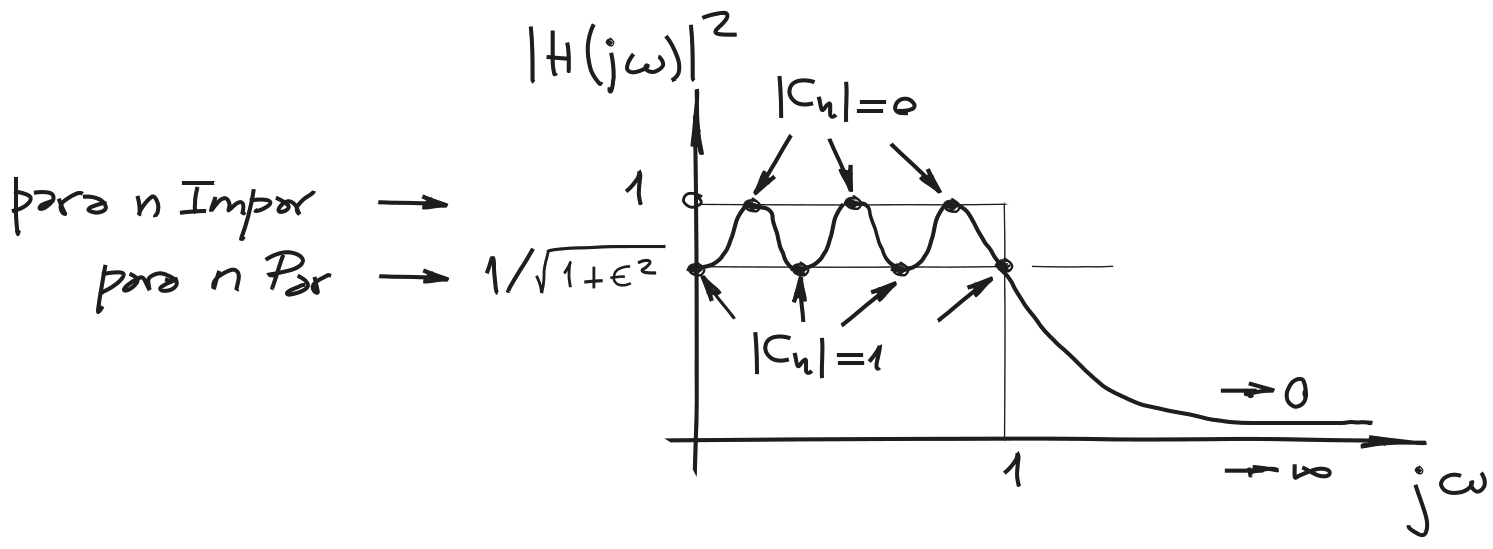
\includegraphics[width=\linewidth]{chebyshev_2.png}
		\caption{Función respuesta en frecuencia del filtro de Chebyshev}
		\end{wrapfigure}				
		&
		Resumen de Propiedades:\newline
		1- Los valores característicos son: 
		
			\[ \left| H(j1) \right|^2 = \frac{1}{1 + \epsilon^2} \mbox{ para todo n }  \] 
			\[ |H(j0)|^2 = \begin{cases}
							1 & \mbox{ para n impar} \\
				            \frac{1}{1+\epsilon^2} & \mbox{ para n par}
							\end{cases}  \]
			
			2- Dentro de la banda de paso, $ 0 \le \omega \le 1 $, $ H(j\omega)$ oscilará entre 1 y $\frac{1}{\sqrt{1+\epsilon^2}}$, entonces la amplitud del riple queda definida por: 
			
				\[ 
					Riple = 1 - \frac{1}{\sqrt{1 + \epsilon^2}}
				 \]			
		\end{tabular} \newline
	
%%	
\textbf{Orden del filtro, constante de riple y atenuación:}\newline	
	
La atenuación esta dada por:  $$ \alpha_n = -10 log_{10} \left| H_n(j\omega) \right|^2 = 10 log \left| 1 + \epsilon^2 C_n^2(\omega) \right| \mbox{ dB}$$ \newline                      

En la banda de rechazo, $ \omega>\omega_c $, siendo $\omega_c$ la frecuencia de corte, la función de aproximación de Chebyshev es $C_n(\omega)=cosh(n \cdot cosh^{-1}) \omega)) $ y por lo tanto la atenuación en esta banda es:
	
	\begin{equation}
		\label{eqn:func:att}	
		\alpha_n = 10 log \left| 1 + \epsilon^2 cosh^2( n \cdot cosh^{-1} \omega) \right| \mbox{ dB}
	\end{equation}
	
donde es dependiente de la constante de riple $\epsilon$ y del orden $n$.\newline
	
Además, el \underline{orden $n_s$} requerido para la \underline{mínima atenuación} deseada en la banda de rechazo se despeja evaluando la ecuación \ref{eqn:func:att} en $\omega_s$:

			$$ n_s = \frac{ cosh^{-1}  \left(
						   \frac{ \sqrt{ 10^{A_{dB}/10}-1} }{\epsilon} 
						               \right)
						  }{ cosh^{-1}( \omega_s ) } $$

De igual forma, el \underline{orden $n_{3db}$} requerido en la frecuencia de corte (con atenuación 3dB), $\omega_c$, es: 
			$$ n_{3dB} = \frac{ cosh^{-1}  \left(
						   \frac{ \sqrt{ 10^{3_{dB}/10}-1} }{\epsilon} 
						               \right)
						  }{ cosh^{-1}( \omega_c ) } $$	
					  
El orden del filtro se estima como el máximo orden que cumpla los requerimientos de atenuación dados.
			$$n=max(n_s, n_{3dB})$$
	
El \underline{riple} se despeja de la atenuación máxima deseable en la banda de paso, en $H(j1)$, y es:
					$$\alpha_{max}=10 log_{10} ( 1 + \epsilon^2 )$$
quedando que el riple definido por:
	   			$$\epsilon = \sqrt{10^{\alpha_{max}/10} - 1} $$	
   			
\underline{Desarrollo:}\newline
	\begin{center}
	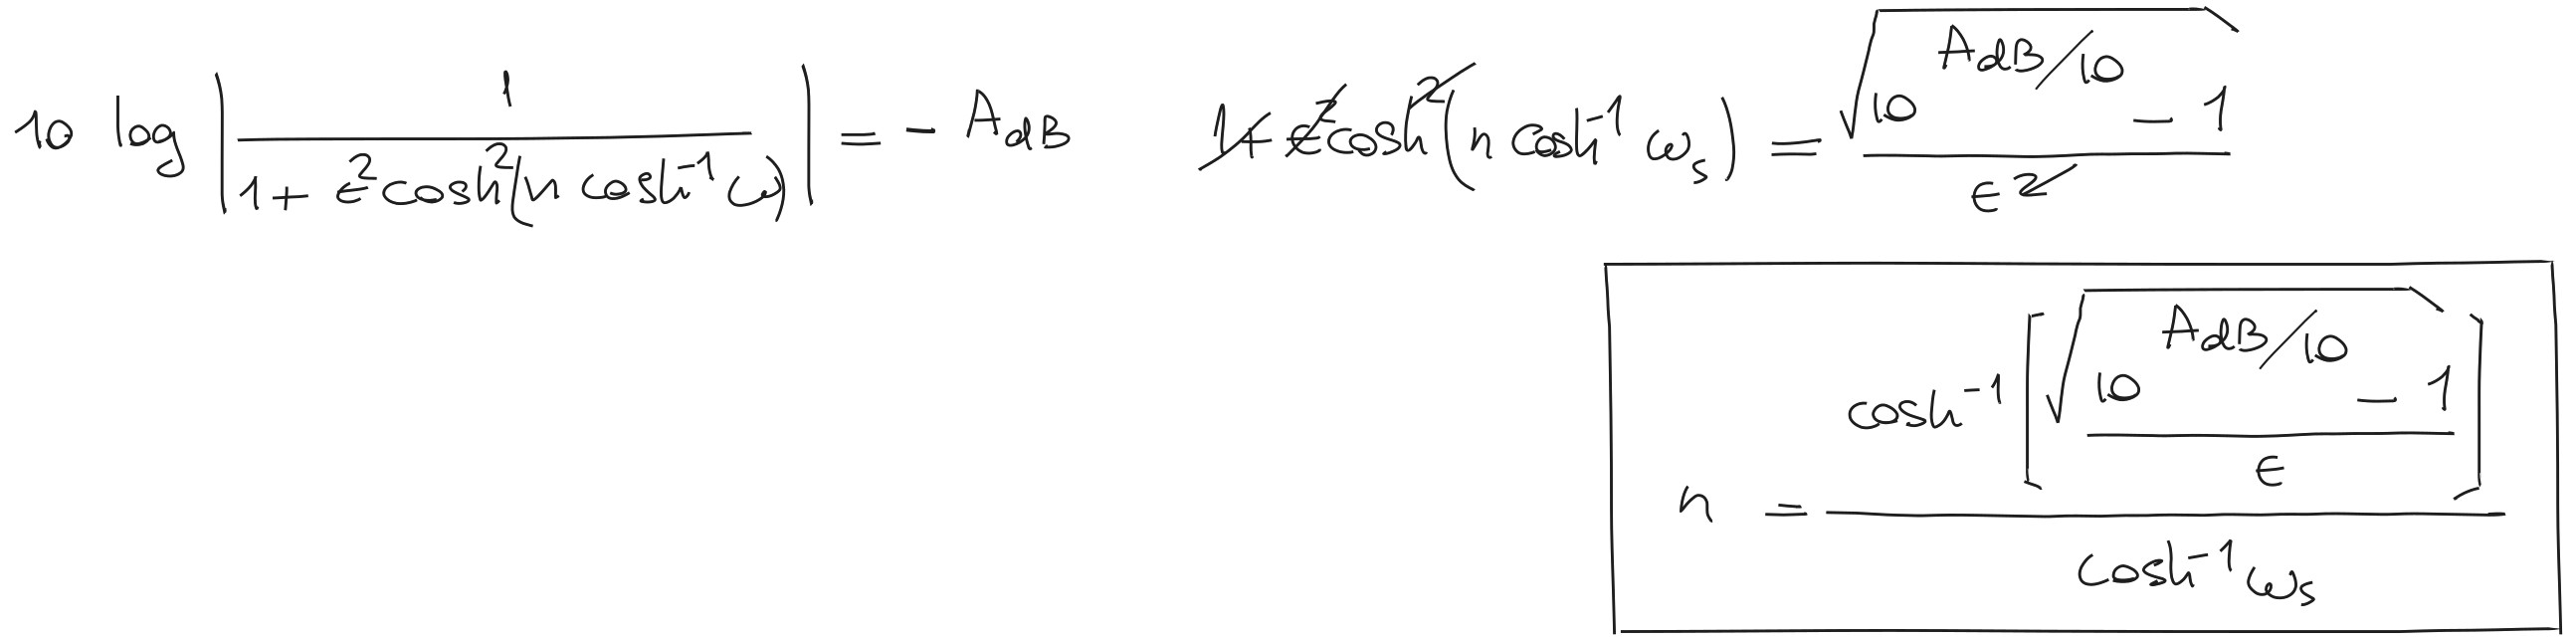
\includegraphics[scale=0.6]{chebyshev_3_orden.jpg}
	\end{center}


\textbf{Función de transferencia a partir de los polos }\newline

La función de transferencia va a ser una función racional de variable compleja s y va a tener la forma
	
	$$H(s)= \prod_{k=1}^{n} \frac{1}{s-s_k}$$
	
donde $s_k$	son polos ubicados en el semiplano izquierdo, $k$ son valores enteros definidos desde $k=1, ... , n$, donde $n$ es el orden del filtro y $s_k = (\sigma_k' + j \omega_k')  cosh( \beta_k)$ evaluada en $k=1,2,...,n$ da  las raíces del denominador, para la cual se tiene que:
	\begin{center}
		$$ \sigma_k' = tanh( \beta_k ) sin \left( \frac{2k-1}{2n} \pi \right)  
		, \omega_k' = cos \left( \frac{2k-1}{2n} \pi \right)  
		, \beta_k = \frac { sinh^{-1}(1 / \epsilon )}{n}$$
	\end{center}

Geométricamente hablando, los polos en el filtro Chebyshev se ubicaran sobre una elipse en el plano s, con el eje mayor sobre el eje imaginario, Fig.\ref{fig:chebyshev:elipse}. Así que cuanto más delgada sea la elipse más influencia tendrán los polos sobre el eje imaginario, y mayor riple.\newline		
	
	\begin{figure}[h!]
		\centering
		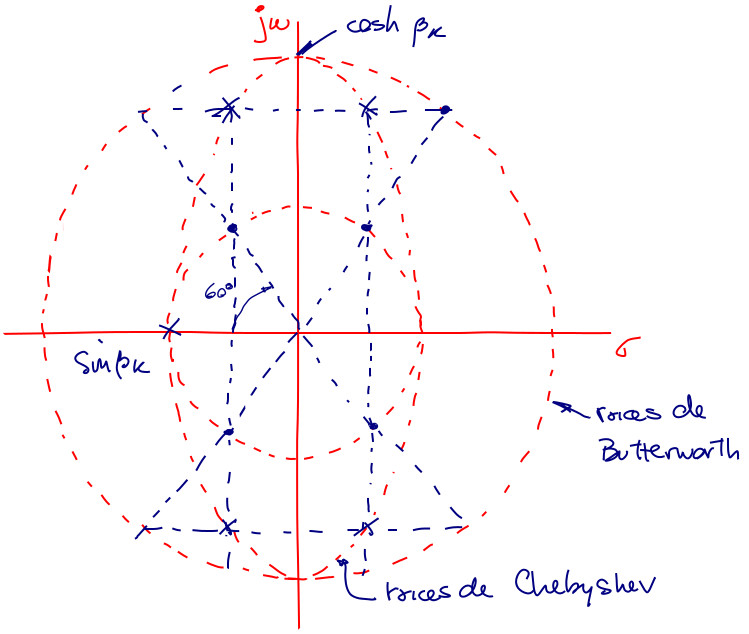
\includegraphics[scale=1.5]{chebyshev_4_elipse.jpg}
		\caption{Ubicación de los polos en el plano imaginario.}
		\label{fig:chebyshev:elipse}
	\end{figure}
	
\underline{Desarrollo del cálculo de las raíces del denominador}:\newline

	Para encontrar los polos se buscan los ceros del denominador, así que primero hay que desarrollar el denominador como sigue: \newline
	\begin{center}
		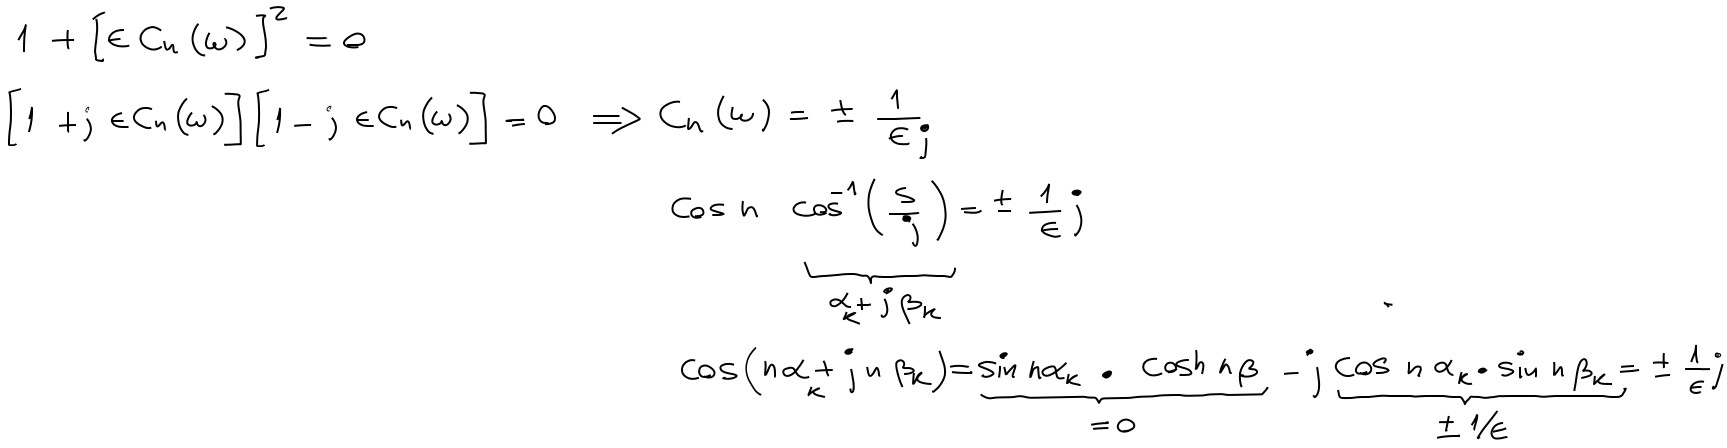
\includegraphics[scale=1]{chebyshev_5_polos_1.jpg}
	\end{center}
	
encontrando como soluciones a \newline
	
	\begin{center}
		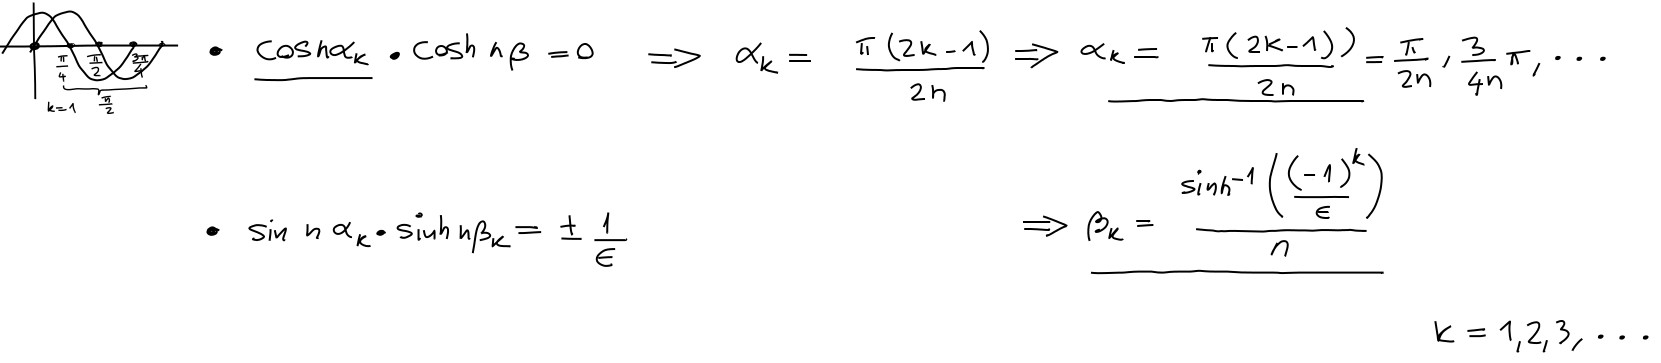
\includegraphics[scale=1.1]{chebyshev_6_polos_2.jpg}
	\end{center}
	
Despejando $s_k$ se tiene:
	
	\begin{center}
		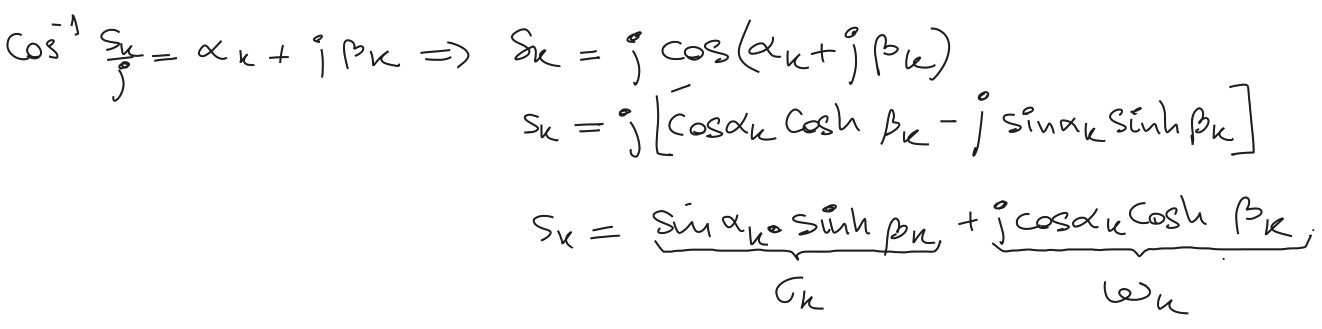
\includegraphics[scale=1]{chebyshev_7_polos_3.jpg}
	\end{center}

	y por identidad trigonométrica, la ubicación geométrica de los polos queda dada en una elipse, tal como se muestra en Fig.\ref{fig:chebyshev:elipse}\newline
	\begin{center}
		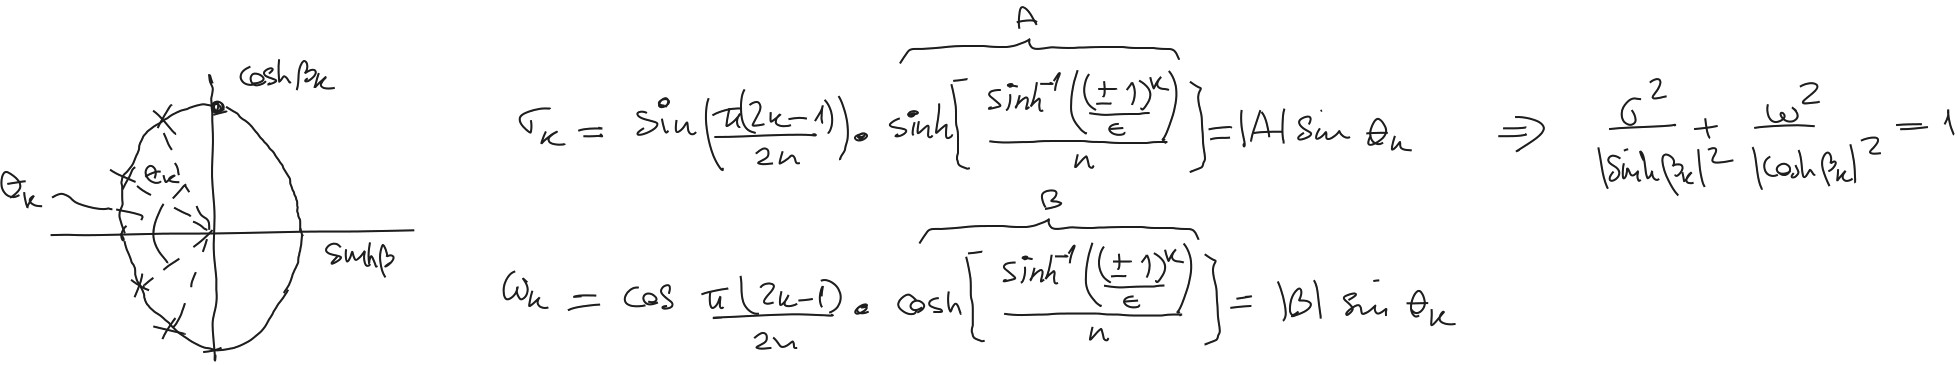
\includegraphics[scale=1]{chebyshev_8_polos_4.jpg}	
	\end{center}

Para compararlo con la geometría de una circunferencia de radio igual a uno, se normalizan las raíces tal como sigue:
	
	\begin{center}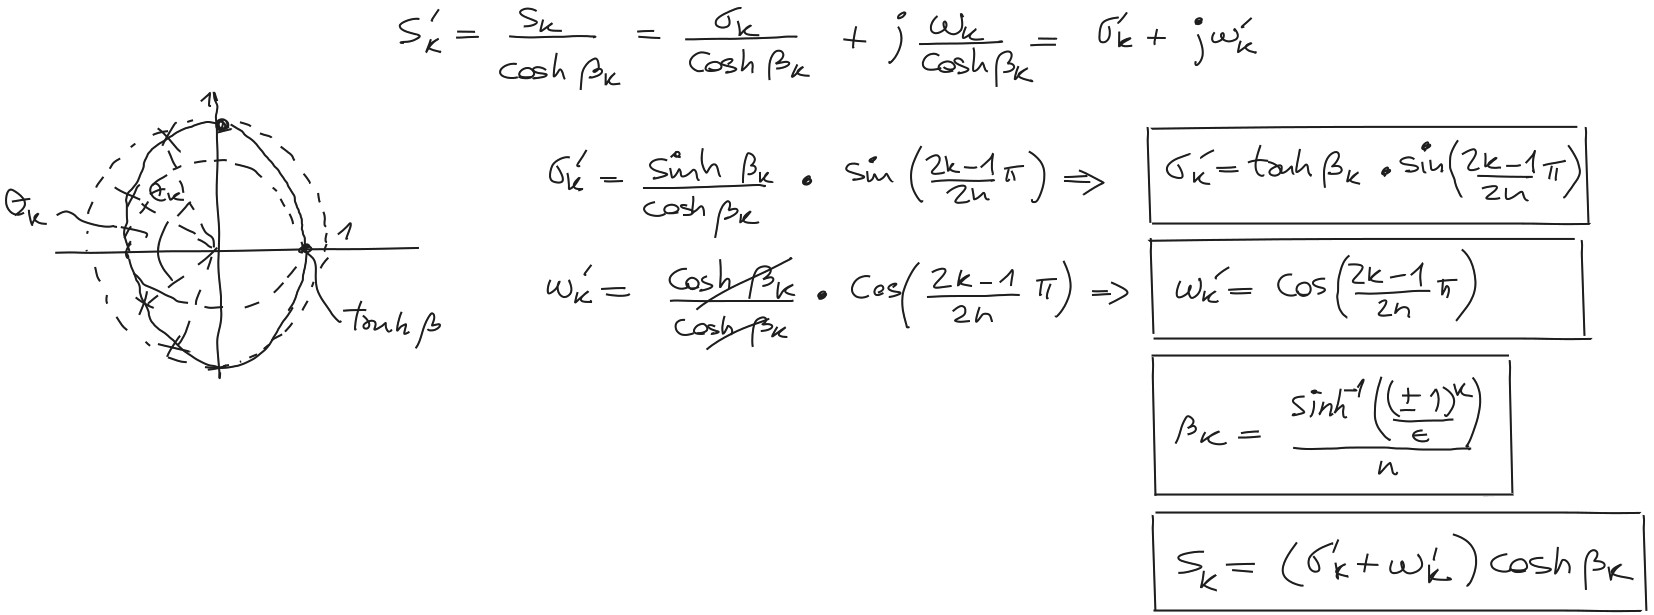
\includegraphics[scale=1]{chebyshev_9_polos_5.jpg}\end{center}		

%%		
\textbf{Ejemplo con Matlab 1:} Determinando los polos y ceros para orden 3, Fig. \ref{fig:func:chebyshev:ej1}.\newline 
  
\lstinputlisting[language=Matlab, frame=single]{./src_matlab/chebyshev_ej1.m}      

En el script se observa que una vez que se tienen los polos, según el orden y constantes de riple dados, se construye muy fácilmente la respuesta en frecuencia del filtro.
    	
	\begin{figure}[h]
		\centering
		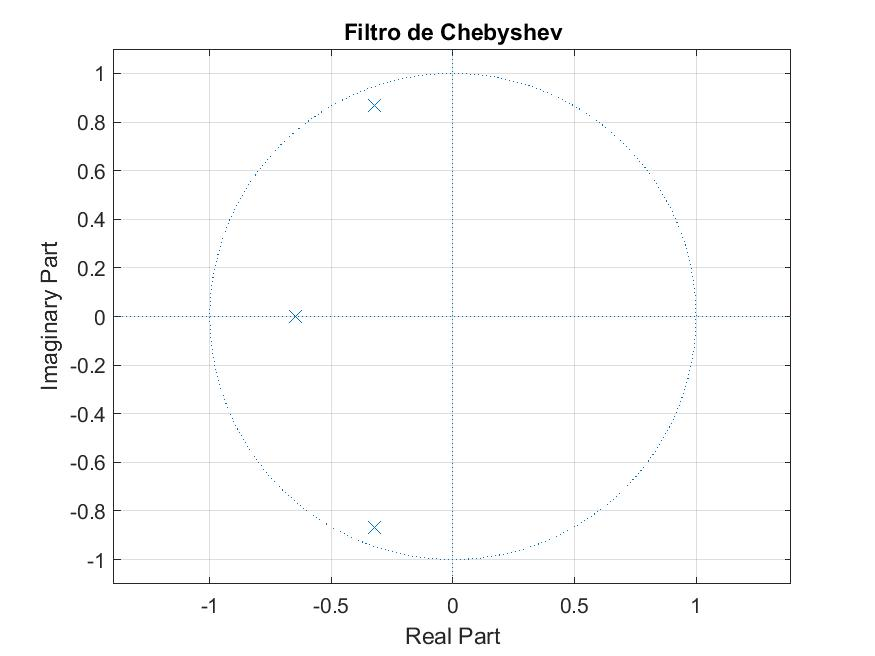
\includegraphics[scale=0.3]{chebyshev_ej1_pz.jpg}
		\caption{Diagrama de polos y ceros del filtro de Chebyshev del ejemplo 1}
		\label{fig:func:chebyshev:ej1}
	\end{figure}
	
%%		
\textbf{\newpage Ejemplo con Matlab 2:} Filtro pasa bajo de Chebyshev a partir de las especificaciones dadas, Fig. \ref{fig:func:chebyshev:ej2}. \newline 
  
Primero, se define una función que determine el orden y la constante de riple requerido para las características prefijadas del filtro a diseñar.\newline
 
\lstinputlisting[language=Matlab, frame=single]{./src_matlab/mi_cheb1ord.m}   
   
El procedimiento para el diseño del filtro es similar al realizado en el Ejemplo 1, la diferencia radica en que se determina el orden  y la constante de riple a partir de los requerimientos propuestos para este ejemplo.
   
\lstinputlisting[language=Matlab, frame=single]{./src_matlab/chebyshev_ej2.m}     
    	
\begin{figure}[h]
     \centering
     \begin{subfigure}[b]{1\textwidth}
         \centering
         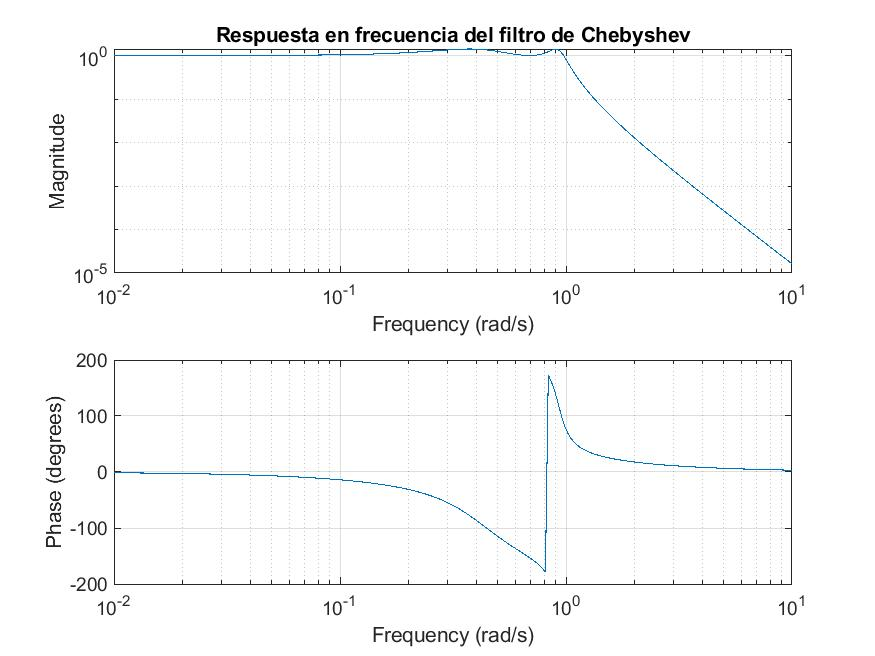
\includegraphics[scale=0.35]{chebyshev_ej2_freqs.jpg}
         \caption{Respuesta en frecuencia del filtro Chebyshev del Ejemplo 2}
         \label{fig:func:chebyshev:ej2:freqs_bp}
     \end{subfigure}
     \bigskip
     \begin{subfigure}[b]{1\textwidth}
         \centering
         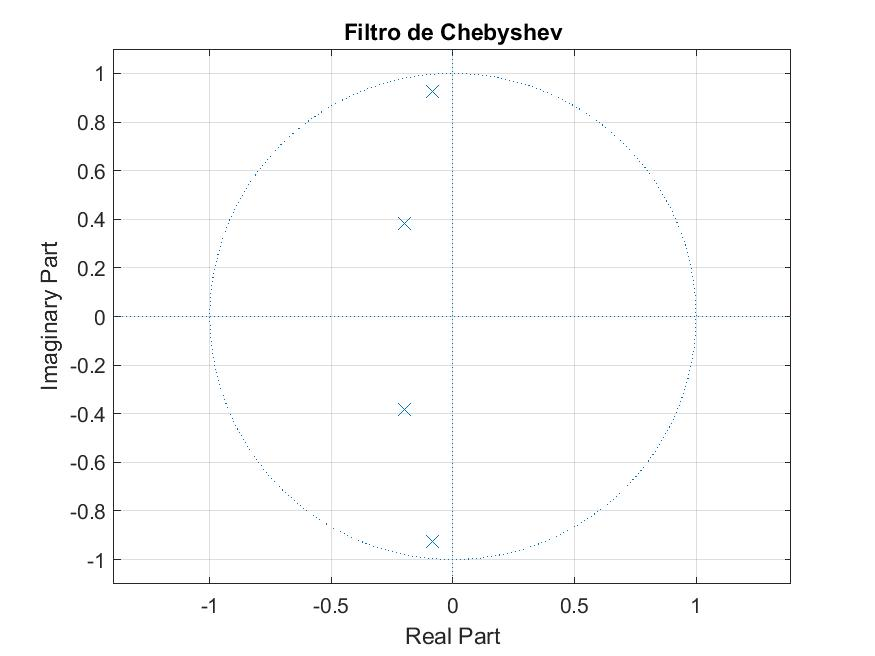
\includegraphics[scale=0.35]{chebyshev_ej2_pz.jpg}
         \caption{Diagrama de polos y ceros del filtro de Chebyshev del Ejemplo 2}
         \label{fig:func:chebyshev:ej2:pz}
     \end{subfigure}
     \caption{Ejemplo 2}
     \label{fig:func:chebyshev:ej2}
\end{figure}

	
\end{document}
